%%%%%%%%%%%%%%%%%%%%%%%%%%%%%%%%%%%%%%%%%%%%%%%%%%%%%%%%%%%%%%%%%%%%%%
%
\section{IVT-specific commands}
%
%%%%%%%%%%%%%%%%%%%%%%%%%%%%%%%%%%%%%%%%%%%%%%%%%%%%%%%%%%%%%%%%%%%%%%

This section defines the
special commands that are available only at the IVT environment.
Those special commands
react on different layouts defined in the environment,
thus making it convenient to switch between paper layouts.

%%%%%%%%%%%%%%%%%%%%%%%%%%%%%%%%%%%%%%%%%%%%%%%%%%%%%%%%%%%%%%%%%%%%%%
\subsection{Figures} \label{sec:compStructs-Figures}
%%%%%%%%%%%%%%%%%%%%%%%%%%%%%%%%%%%%%%%%%%%%%%%%%%%%%%%%%%%%%%%%%%%%%%

There are three commands for including Figures. One for a single Figure
and one for a Multi-Figure. The position of the Figure is chosen by
\LaTeX,
but a hint can be provided.

\subsubsection{Single Figures}

\label{sec:compStructs-Figures-SingleFigures}

A single figure as shown in \cref{fig:labelOfTheSingleFigure}
has the following construct:

\textbackslash{}createfigure[\ref{item:singFig0}]\{\ref{item:singFig1}\}\{\ref{item:singFig2}\}\{\ref{item:singFig3}\}\{\ref{item:singFig4}\}\{\ref{item:singFig5}\}
\begin{enumerate}
  \item\label{item:singFig0} the placement modifier (optional)
  \item\label{item:singFig1} the short caption for the content List
  \item\label{item:singFig2} the long caption shown next to the figure
  \item\label{item:singFig3} the label of the figure
  \item\label{item:singFig4} the figure
  \item\label{item:singFig5} the source with other additional comments
\end{enumerate}

The placement modifier (item~\ref{item:singFig0})
specifies where the figure appears in the final document.
It can be ``tp'', ``htp'' or ``hp'';
``t'' means ``at the top of this or a following page'',
``h'' means ``at the place where the command appears'',
and ``p'' means ``on a separate page''.
If you leave out this parameter (including the square brackets),
``tp'' is the default.
Usually a figure will appear on the next suitable location
after it has been declared.
The placement on a separate page will be used as a last resort
if the figure does not fit anywhere else, even if you do not include it.

If the short and the long caption
(item~\ref{item:singFig1}\&\ref{item:singFig2}) should say the same,
just add the same text twice. Item~\ref{item:singFig3} ALWAYS defines
a label (as shown in \cref{sec:compStructs-LabelsCrossRefs}).
Item~\ref{item:singFig4} always contains the ``\textbackslash{}includegraphics''
command. The parameter ``width'' defines the size of the Figure
(respecting width and length ratio). If ``width'' is equal to
1.0\textbackslash{}textwidth the Figure has width of the text area width.
With ``angle'' you can rotate the Figure (+/-180).
With Item~\ref{item:singFig5} you can add a source. If you do not want
to add a source, just leave it empty. If not, ``Source: '' or
``Quelle: '' will be added followed by your text.

%---------------------------------------------------------------------
\createfigure%
{Single Figure: Short Caption (for the Content)}%
{Single Figure: Here you can add the long Caption of the Figure. This
Caption apprears only in the paper and NOT in the Content. With that,
the content list is much better to read. The Caption for the Content
can be added above.}%
{\label{fig:labelOfTheSingleFigure}}%
{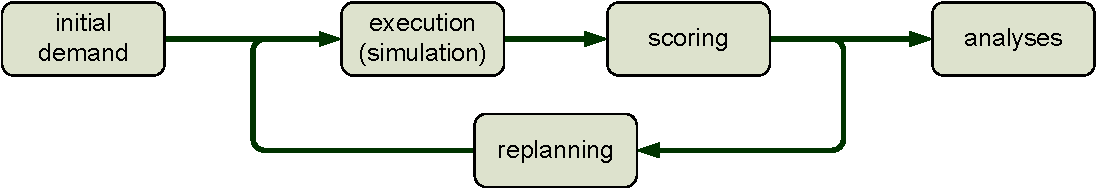
\includegraphics[width=1.0\textwidth, angle=90]{figures/MATSimLoop}}%
{Christoph Dobler}
%---------------------------------------------------------------------

\subsubsection{Multi-Figures}

Multi-Figures uses the same command as for single Figures. But instead
of adding one  ``\textbackslash{}includegraphics'' command in Item~\ref{item:singFig4}
you can add as many ``\textbackslash{}createsubfigure'' commands as you want.

The structure of the ``\textbackslash{}createsubfigure'' command is:
\begin{enumerate}
  \item\label{item:multFig1} the caption for the sub-figure
  \item\label{item:multFig2} the figure (again by using the
``\textbackslash{}includegraphics'' command)
  \item\label{item:multFig3} the label of the sub-figure
  \item\label{item:multFig4} either \textbackslash{}\textbackslash{} or leave it
empty
\end{enumerate}
The last item defines, if you want a line break between this
sub-figure and the following one. By using \textbackslash{}\textbackslash{} the
following figure will be on the next line. The last Sub-Figure should
not use \textbackslash{}\textbackslash{}.

\Cref{fig:labelOfTheMultiFigure1} contains two sub-figures
(\cref{fig:labelOfTheMultiFigure1-SubFig1,fig:labelOfTheMultiFigure1-SubFig2}) put on the same
line.

%---------------------------------------------------------------------
\createfigure%
{Multi-Figure1: Short Caption}%
{Multi-Figure1: Long Caption}%
{\label{fig:labelOfTheMultiFigure1}}%
{%
  \createsubfigure%
  {Caption of the first Sub-Figure}%
  {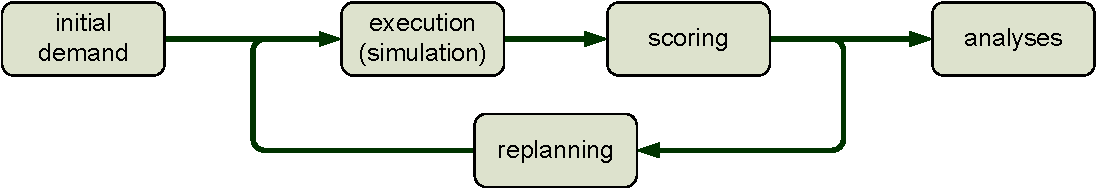
\includegraphics[width=0.49\textwidth,
angle=0]{figures/MATSimLoop}}%
  {\label{fig:labelOfTheMultiFigure1-SubFig1}}%
  {}%
  \createsubfigure%
  {Caption of the second Sub-Figure}%
  {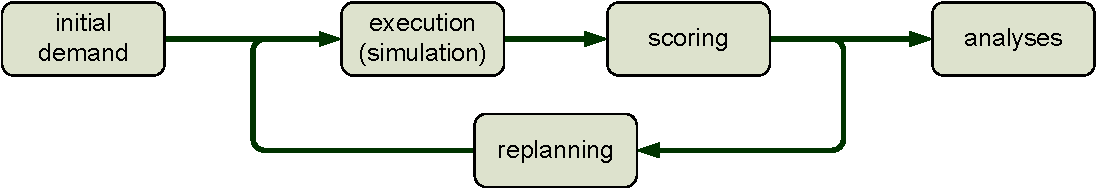
\includegraphics[width=0.49\textwidth,
angle=0]{figures/MATSimLoop}}%
  {\label{fig:labelOfTheMultiFigure1-SubFig2}}%
  {}%
}%
{}
%---------------------------------------------------------------------

\Cref{fig:labelOfTheMultiFigure2} contains three sub-figures
(\cref{fig:labelOfTheMultiFigure2-SubFig1,fig:labelOfTheMultiFigure2-SubFig2,fig:labelOfTheMultiFigure2-SubFig3}). The first one is set
on the first line, while the other two are set to the second line.

%---------------------------------------------------------------------
\createfigure%
{Multi-Figure2: Short Caption}%
{Multi-Figure2: Long Caption}%
{\label{fig:labelOfTheMultiFigure2}}%
{%
  \createsubfigure%
  {Caption of the first Sub-Figure}%
  {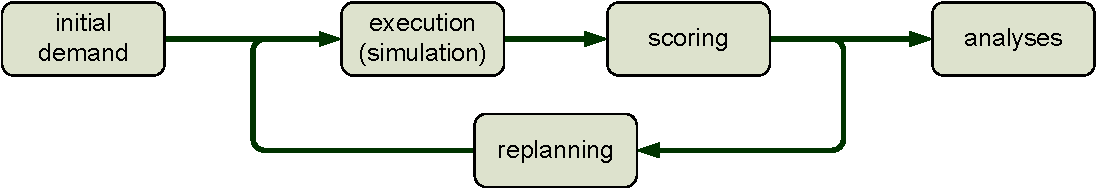
\includegraphics[width=0.70\textwidth,
angle=0]{figures/MATSimLoop}}%
  {\label{fig:labelOfTheMultiFigure2-SubFig1}}%
  {\\}%
  \createsubfigure%
  {Caption of the second Sub-Figure}%
  {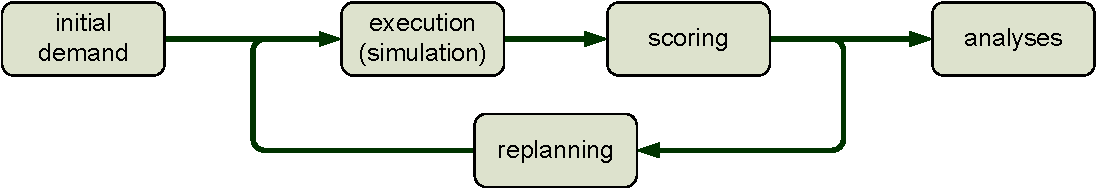
\includegraphics[width=0.48\textwidth,
angle=0]{figures/MATSimLoop}}%
  {\label{fig:labelOfTheMultiFigure2-SubFig2}}%
  {\hfill}%
  \createsubfigure%
  {Caption of the third Sub-Figure}%
  {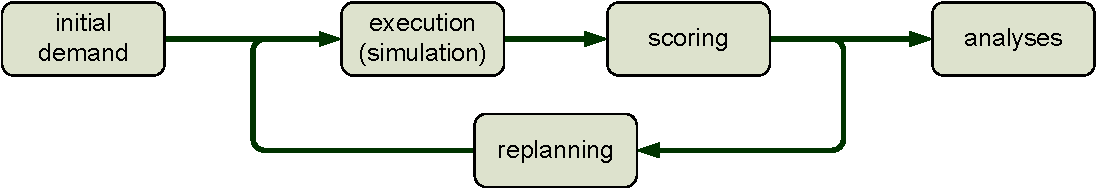
\includegraphics[width=0.48\textwidth,
angle=0]{figures/MATSimLoop}}%
  {\label{fig:labelOfTheMultiFigure2-SubFig3}}%
  {}%
}%
{my source}
%---------------------------------------------------------------------

\subsubsection{Landscape figures}

Oversize figures in landscape orientation can be put rotated
on a separate page
using the ``\textbackslash{}createsidewaysfigure''
command,
only that no placement specifier is available.
The syntax is identical to that of the
``\textbackslash{}createfigure''
command (cf.~\cref{sec:compStructs-Figures-SingleFigures}).
The page is rotated for on-screen display, too.
The result can be seen in \cref{fig:loop-page}.
\createsidewaysfigure{%
MATSim simulation loop}{%
The MATSim simulation loop}{%
% Used when referring to the figure
\label{fig:loop-page}%
}
{%
% Command that loads the figure.
% Supported formats: PDF, PNG and JPEG.
% File extension can be omitted
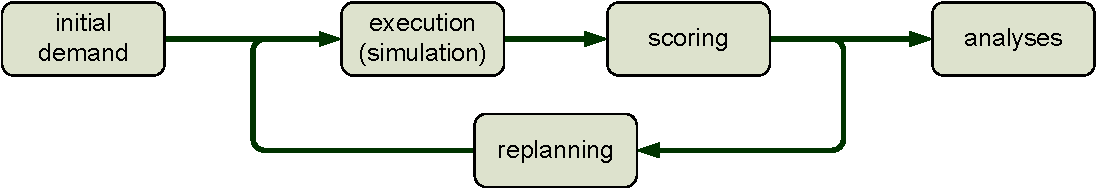
\includegraphics[width=\linewidth]{figures/MATSimLoop}%
}{%
% The source (now mandatory, but can be empty)
Christoph Dobler%
}


%%%%%%%%%%%%%%%%%%%%%%%%%%%%%%%%%%%%%%%%%%%%%%%%%%%%%%%%%%%%%%%%%%%%%%
\subsection{Tables} \label{sec:compStructs-Tables}
%%%%%%%%%%%%%%%%%%%%%%%%%%%%%%%%%%%%%%%%%%%%%%%%%%%%%%%%%%%%%%%%%%%%%%

A table has the same structure as the single Figure (see above). But
instead of including a graphic in item~4 you add the ``tabular''
construct. Unfortunately it is not that easy to understand and edit such a table. One has
to get used to it. However, quite a few tools can help converting the data
to the \LaTeX{} format, see \url{http://tex.stackexchange.com/q/49414/8057}
for an overview.

If you do not like it you can still add the table
as a graphic (with the ``\textbackslash{}includegraphics'') command.
But you still need to use the ``\textbackslash{}createtable'' command,
otherwise your table will appear
in the list of figures instead of the list of tables.
\Cref{tab:labelOfTheTable} shows an example of a table.

%---------------------------------------------------------------------
\createtable%
{A Tables short Caption}%
{A Tables long Caption}%
{\label{tab:labelOfTheTable}}%
{%
  \begin{tabular}[c]{lr@{.}lcr@{.}l}
    \toprule
    Bias / Error     & \multicolumn{2}{c}{Routes Only} &
\multicolumn{3}{c}{Times and Routes} \\
    \midrule
    Mean Abs. Bias:  & $+$331&40                        && $+$306&32  
                         \\
    Mean Rel. Bias:  &  $+$19&62\%                      &&  $+$25&27\%
                         \\
    \midrule
    Mean Abs. Error: &    533&55                        &&    503&77  
                         \\
    Mean Rel. Error: &     37&50\%                      &&     35&38\%
                         \\
    \bottomrule
  \end{tabular}
}%
{my source}
%---------------------------------------------------------------------

There is an analogous command ``\textbackslash{}createsubtable'' for multi-tables.

%%%%%%%%%%%%%%%%%%%%%%%%%%%%%%%%%%%%%%%%%%%%%%%%%%%%%%%%%%%%%%%%%%%%%%
\subsection{Pretty Printing}
%%%%%%%%%%%%%%%%%%%%%%%%%%%%%%%%%%%%%%%%%%%%%%%%%%%%%%%%%%%%%%%%%%%%%%

\LaTeX{} provides several functionalities for printing nice code, data
and so on. At the moment the layout features a nice way of printing
XML code. You do not have to copy XML into this paper, instead you can
include an XML file.
The command is similar to the Figure (it also will be included into
the list of figures). \Cref{fig:xml-plan} shows an example.

%---------------------------------------------------------------------
\createxmlfigure%
{A typical plan in XML.}%
{A typical plan in XML. This agent, id 393241, leaves home (on link
id 5834 of the given network) at 7:00~AM (performing home activity
for 7~hours), and drives to work via a four-node route (five links)
which it expects to take 25~minutes to traverse.  The agent stays at
work for 9~hours, then drives home again via a two-node route and
stays at home until midnight. Therefore, it describes a complete
day-plan for person number 393241.}%
{\label{fig:xml-plan}}%
{listings/examplePlans.xml}%
{}
%---------------------------------------------------------------------

If you want other pretty printing options, please ask
kirill.mueller@ivt.baug.ethz.ch.

